\documentclass[]{article}

\usepackage{graphicx}
\usepackage{float}
\usepackage[a4paper,top=2.5cm,bottom=2.5cm,left=2.5cm,right=2cm]{geometry}
\usepackage{subcaption}
\usepackage[table,xcdraw]{xcolor}
\usepackage{makecell}

\setlength{\tabcolsep}{13pt}
\renewcommand{\arraystretch}{2.3}

\title{ RASD \\
	\begin{large} 
		Software Engineering 2
	\end{large}}

\author{Antonio Ercolani - 10621728\\Vittorio Fabris - 10562731\\Riccardo Nannini - 10626268}
\date{Academic year 2020/2021}


\begin{document}
	\pagenumbering{gobble}
	
	\maketitle
	\begin{paragraph}
		\newline
	\end{paragraph}

	\newpage
	\pagenumbering{arabic}	


	\tableofcontents
	
	\newpage
	
	
	\section{Introduction}
	
	\subsection{Purpose}
	
	The \textit{Requirement Analysis and Specification Document} (RASD) is a standardized document used by software engineers to communicate the most important aspects of a system to be developed to the project stakeholders. The RASD represents the starting point of the so called “waterfall life-cycle” of a software system, therefore it’s easy to understand how delicate and strategical is the role it performs. Programmers, testers, designers and everyone involved in the development will refer to this paper and a mistake could potentially cost thousand hours of additional work. 
	\smallskip
	\\
	What we said so far is the purpose of this document. This specific RASD is about an application that tries to face the crowding of supermarkets during the coronavirus emergency. In the following section we are going to explain the scope of that software system.

	\subsection{Scope}
	
		\begin{paragraph}
			\newline
				The scope of the software is to give the users the possibility to line up to enter and shop into a grocery stores.\\
				The stores that have registered to this service generate and distribute tickets to line people correctly, letting them do the shopping only if the QR-code scanned on their ticket is valid.\\
				CLup offers different kind of functionalities and features:\\
	
			\begin{itemize}
			\item \textbf{Basic:}
				The user can line up in different ways: through a physical ticket taken outside the store, or through the application, that is implemented in a way such that people of every age can use. \\
				If there are already too many people queuing outside the shop, the software doesn’t allow to distribute new physical tickets. \\
				The software can integrate the information derived  from the two sources, virtual and physical bookings, so that overcrowding is avoided in the neighborhood of the store and thanks to the QR ticket validations, store managers can monitor entrances. \\
				When the user leaves the store he must show his ticket to the QR-reader again, so that the system can know it and let the queue proceed, with another customer enter the shop.\\

			\item \textbf{Feature 1:}
				Users that line up from home concede the system to see where they are, using the GPS position of their device to identify their zone. In this way only nearby grocery stores are shown to the user.\\
				What’s more, these category of users can book a visit at a specific time, if there is a free spot in the schedule organized by the system, otherwise other arrival times or grocery stores are proposed to the user.\\
				The system, knowing the position of the user, his distance from the store and the vehicle that he has chosen to use to reach it, will provide him a notification that in a certain moment he should leave to arrive on time at the grocery store. If the user arrives late, the system can reschedule a booking for him, always considering to avoid overcrowding and the time preferences of the customer, inserting him into the line again.\\

			\item  \textbf{Feature 2:}
				Because the system needs to balance in the best way possible the number of people inside the store, the user that books online his visit is also asked which kind of products he’s going to buy. In this way the system can manage people along the store’s aisles, reducing the possible interaction and proximity of customers, distributing their access into the shop in different times if it is necessary.  \\

			\item  \textbf{Feature 3:}
				When the grocery store registers to the service, it can decide if he wants to save the information about the preferences of customers about the products they buy. In fact, as explained in the previous feature, the user lets the system know what he intends to buy. The grocery store could use these preferences in order to manage a plan for the refill of its shelves and always be ready to satisfy the needs of  its customers, avoiding the risk of not having some products to sell, but ordering them from their providers in advance.

			\end{itemize}
			
	
		\end{paragraph}
	
		\subsubsection{World phenomena}

			\begin{tabular}{|c|l|}
				\hline
				\rowcolor[HTML]{DCDCDC} 
				\textbf{WP1} & The customer arrives to the store \\ \hline
				\textbf{WP2} & The customer shops in the store \\ \hline
				\rowcolor[HTML]{DCDCDC} 
				\textbf{WP3} & The customer waits outside the store \\ \hline
			\end{tabular}
			
		\subsubsection{Shared phenomena}
		
			Controlled by the \textbf{machine}\newline\newline
					\begin{tabular}{|c|l|}
						\hline
						\rowcolor[HTML]{DCDCDC} 
						\textbf{SP1} & The customer is notified that his turn is coming \\ \hline
						\textbf{SP2} & The store generates and sends a ticket to the user (?) \\ \hline
					\end{tabular} \newline\newline\newline
			Controlled by the \textbf{world}\newline\newline
					\begin{tabular}{|c|l|}
						\hline
						\rowcolor[HTML]{DCDCDC} 
						\textbf{SP3} & The customer enters the store scanning his QR code \\ \hline
						\textbf{SP4} & The customer reserves a place in the queue of a given store using the application \\ \hline
						\rowcolor[HTML]{DCDCDC} 
						\textbf{SP5} & \makecell[l]{The customer reserves a place in the queue of a given store using the ticket totem \\outside the store}\\ \hline
						\textbf{SP6} & The customer books a visit to the store \\ \hline
						\rowcolor[HTML]{DCDCDC} 
						\textbf{SP7} & The customer leaves the store \\ \hline
						\textbf{SP8} & The store receives a request to join its queue \\ \hline
					\end{tabular}
					
		
		\subsubsection{Goals}
		
		\begin{tabular}{|c|l|}
						\hline
						\rowcolor[HTML]{DCDCDC} 
						\textbf{G1} & \makecell[l]{At any time the number of people in the store must not be higher than the store limit or \\ the limit is passed but the customers are expected to be in different areas of the store} \\ \hline
						\textbf{G2} & The physical queue of people outside the store is reduced \\ \hline
						\rowcolor[HTML]{DCDCDC} 
						\textbf{G3} & Allow users to "line up" for a store from home \\ \hline
						\textbf{G4} & Allow users to wait for their turn at home and receive an alert when their turn is coming \\ \hline		
						\rowcolor[HTML]{DCDCDC} 
						\textbf{G5} & Allow users to book a visit to a store \\ \hline
						\textbf{G6} & Balance the number of people between different store or timeframes with suggestions \\ \hline		
						\rowcolor[HTML]{DCDCDC} 
						\textbf{G7} & Allow the store to monitor entries \\ \hline
						\textbf{G8} & Handle the order of entries between the queue and the booked visits \\ \hline	
						\rowcolor[HTML]{DCDCDC} 
						\textbf{G9} & Collects information in order to build statistics and infer mean datas \\ \hline					
					\end{tabular}


	\subsection{Definitions, Acronyms, Abbreviations}
	
	In this section we explain the meaning of some technical terms used in the document.
	\medskip
	\\
	\begin{tabular}{|c|l|}
		\hline
		\rowcolor[HTML]{DCDCDC} 
		\textbf{QR CODE} & \makecell[l]{A \textit{Quick Response code} is a kind of bar-code, readable by machines to retrieve information} \\ \hline
		\textbf{UML} & \makecell[l]{The \textit{Unified Modeling Language} is a modeling language used to describe the design \\of a software system} \\ \hline
	\end{tabular}
	
	
	
	
	\subsection{Revision history}	
	\subsection{Reference Documents}
	
	\subsection{Document Structure}
	
	This RASD document is structured over 6 main chapters, described below.
	
	\paragraph{Chapter 1} starts with a brief description of the purpose of this document. Then the focus moves on the involved software system, for which is given an overall description of the goals, scope and related phenomena. The chapter ends with secondary sections about the description of technical terms and the history of this RASD document.
	
	\paragraph{Chapter 2} let the reader to better understand the "world" of the analyzed software system. It begins with a UML and then other kind of diagrams that explain how the application interact with the environment around it. The following sections are about the requirements the system must satisfy, also with a focus on the specific users needs. Finally, in the last section, we list the domain assumption we did.
	
	\paragraph{Chapter 3} goes deep into the topics described in the previous chapter.
	Begins with the description of the user interface and continue with use cases and sequence diagrams to show how the system behaves in different situations, in respect to the application requirements. Then you will find sections on other system constraints on performance and design. The chapter ends with few words on non-functional requirements.
	
	\paragraph{Chapter 4} tries to describe the main aspects of the software system we have seen so far with an alloy model.
	
	\paragraph{Chapters 5 and 6} contain, respectively, an outline of the effort spent in the project by each team mates and the document references.
	
	\newpage
	\section{Overall description}
	
		\subsection{Product perspective}
		The CLup system is designed as a complitely new software application. The user side of the software is intended to be used as a mobile application while the store managers are going to interface with the software through a web interface. \newline
		In order to estimate the time needed for the user to reach the store, the application needs to interface with the smartphone's localization system and needs the user to indicate the type of transportation that he is going to use. \newline
		The system will handle client that are not using the application with tickets provided by a ticket totem located outside the store. This machine will act as an interface to the software application. \newline
		Customers using CLup are going to be notified when their turn is coming in order to approach the store while those with a ticket outside the store will monitor a screen extern to the shop in order to know when it's their turn to enter. \newline
		In order to access the store, every customer is required to scan their QR code (either from the application or from the physical ticket) when entering and exiting the store: in both cases the system will activate an automatic door. \newline
		On the other side of the system, store managers are going to be able to monitor and manage the queue of their store as well as programmed visits. \newline
		The below class diagram models the application domain in order to give an overlook on the enviroment where the application is going to work.
		
		\begin{figure}[htp]
			\centering
			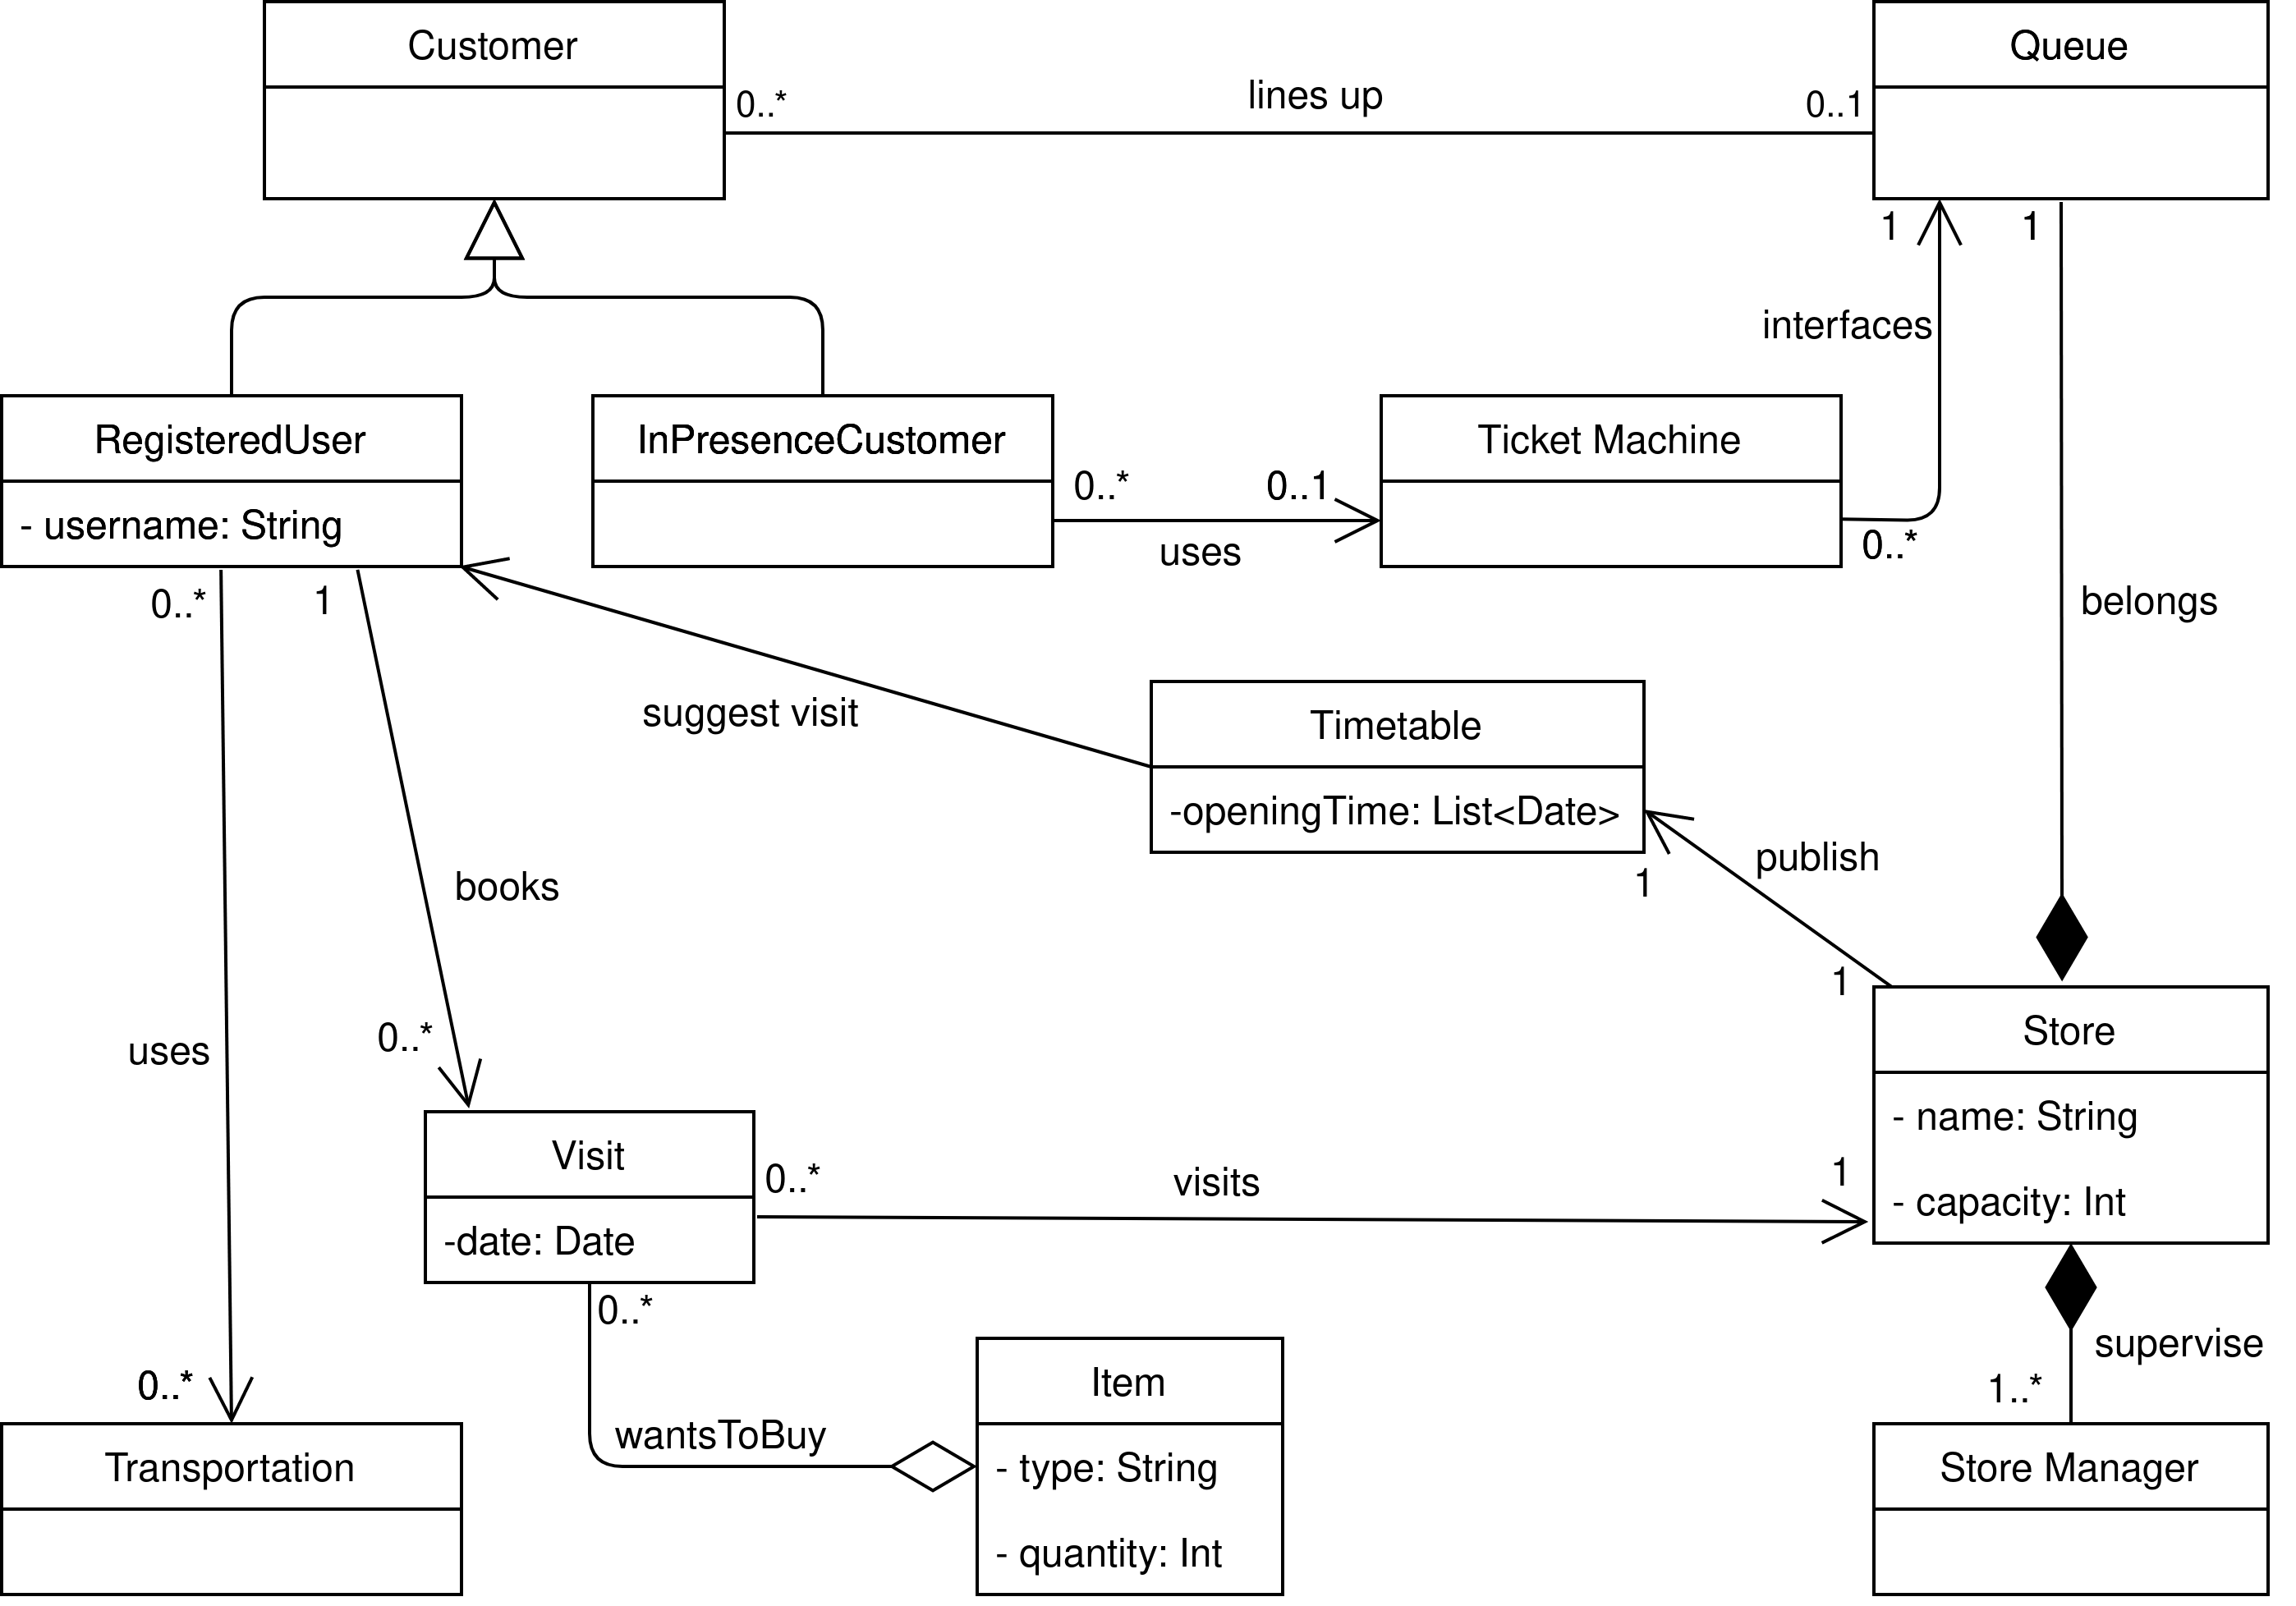
\includegraphics[scale=0.5]{UML_class_diagram.png}
			\caption{Class diagram}
			\label{fig:class_diagram}
		\end{figure}
		
	\textbf{}\\
		\subsection{StateCharts}
		
		\textbf{}\\ \newline
		In this section we want to show the evolution over time of the states of the application and the behavior of the user interacting with the app and the environment. 
The state diagrams below better explain the progress of the system.\\
		
		\textbf{}\\ \newline
		
		\begin{figure}[H]
			\centering
			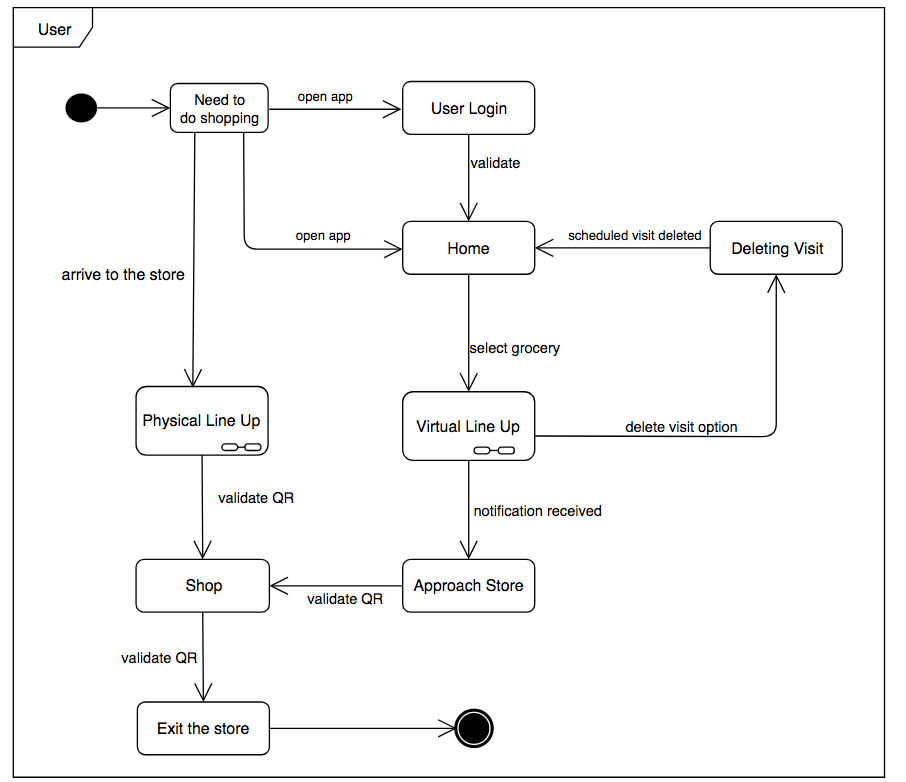
\includegraphics[scale=0.5]{user.png}
			\caption{User State Diagram}
			\label{fig:state_diagram1}
		\end{figure}
		
		
		In the first state diagram (Figure \ref{fig:state_diagram1}) it’s shown how the user interacts with the environment and the system when he needs to do shopping. He interacts with the system lining up to a store in a virtual way using the mobile or web application, or queuing physically at the store he wants to visit.
What’s more, to enter the store, he needs to show the QR-code, and then he has to do the same when he exits, so that the queue can proceed. \\

		\textbf{}\\ \newpage

		\begin{figure}[H]
			\centering
			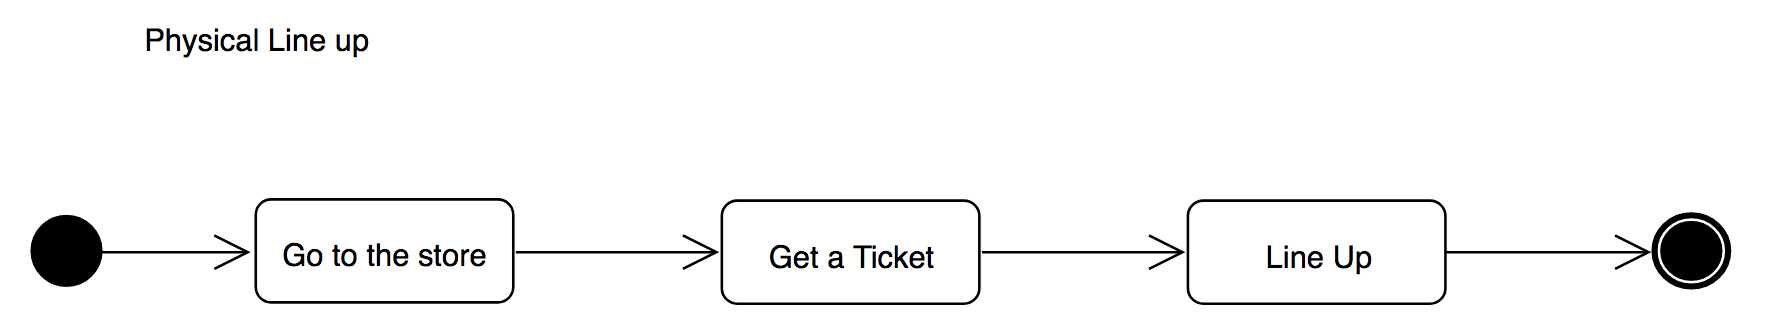
\includegraphics[width=\linewidth]{physicalqueue.png}
			\caption{Physical Line Up State Diagram}
			\label{fig:state_diagram2}
		\end{figure}
		
		
		In this second state diagram (Figure \ref{fig:state_diagram2})  it’s better explained the physical line up of the user, that directly gets a ticket nearby the store.\\
		
		\textbf{}\\ \newline
		\textbf{}\\ \newline
		
		\begin{figure}[H]
			\centering
			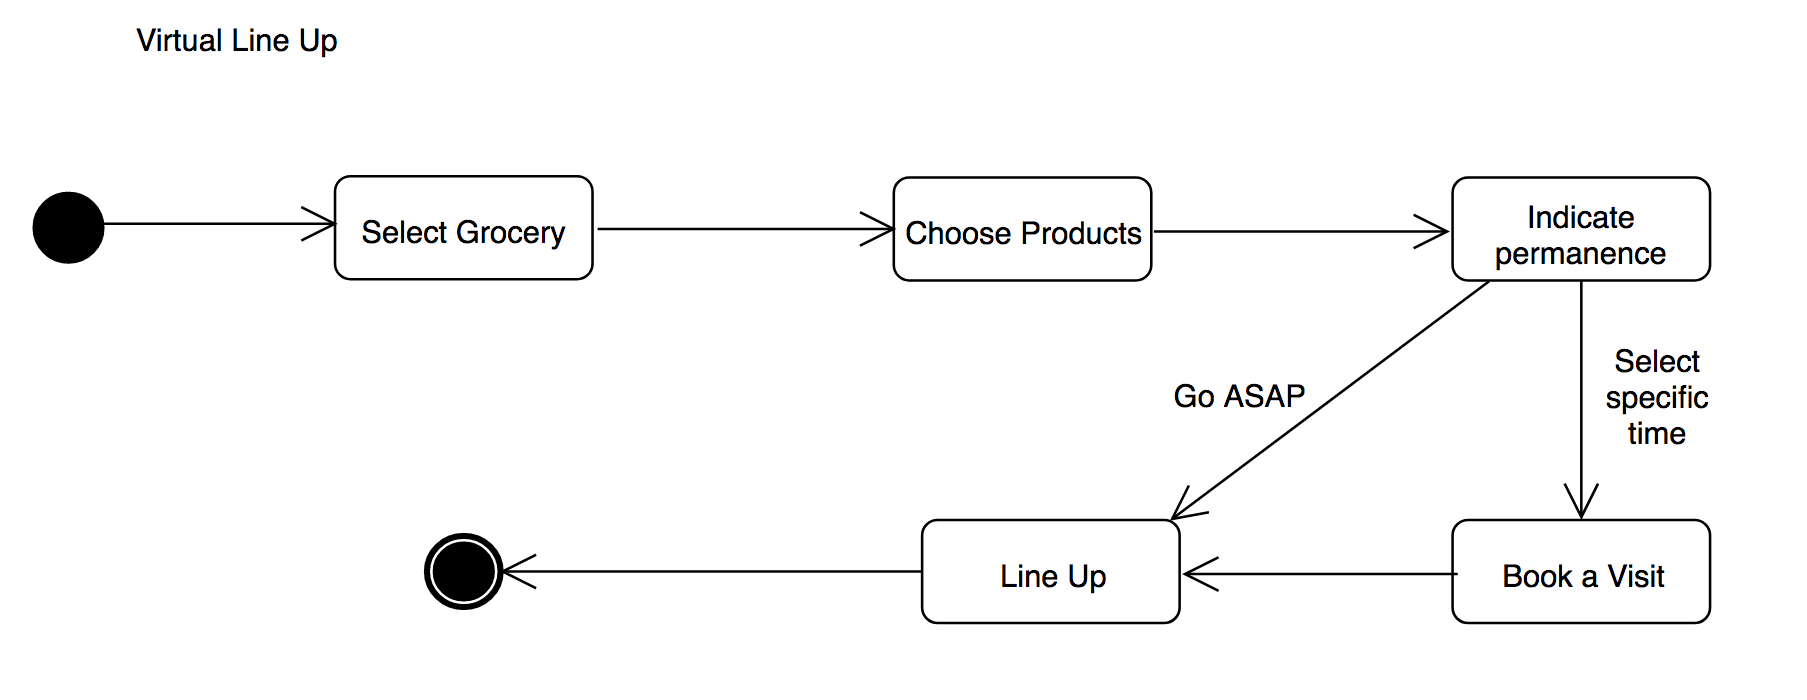
\includegraphics[width=\linewidth]{virtualqueue.png}
			\caption{Virtual Line Up State Diagram}
			\label{fig:state_diagram3}
		\end{figure}
		
		Here (Figure \ref{fig:state_diagram3})  are shown the steps to go through the virtual line up of the user, that has to face some intermediate steps before he gains the possibility to line up to the store. \\
		

\newpage

\subsection{Product functions}

In this section are analyzed the main functionalities that the CLup software system must ensure. Goals and requirements are many and they are all connected with each other, therefore, below you will find the description of two "macro-functionalities" that try to group most of them. Said that, in order to go deeply in every system capability, the reader should supplement this section with the next chapter - "Specific requirements".
\bigskip
\\
\begin{large}
	\textbf{Queue management}
\end{large}
\smallskip
\\
The core function. As the name suggest, the system is able to manage the stores entering queue, that are becoming longer and "dangerous" in the time of coronavirus. This is done with a combination of two sub-functionalities: 

\begin{itemize}
	\renewcommand{\labelitemi}{$-$}
	\item \textbf{Line up from home} - allow users to reserve their place in the queue without having to reach the store, they just need to access the application and choose a grocery. To this simple user action corresponds an important data elaboration made by the system, to ensure another important functionality: \textbf{alert the costumer when his turn comes}. In fact the system must take into account different factors to alert the user in the right moment:
	\begin{itemize}
		\renewcommand{\labelitemi}{$-$}
		\item The distance between the user home and the selected store;
		\item How much time take people before the user in the queue to enter the store.
	\end{itemize} 
	Once the system has collected all the information, it can compute the right amount of time needed by the costumer to reach the store in the right moment he have to enter in.
	\item \textbf{Line up physically} - the system must give the possibility to line up physically. Therefore, when costumers reserve their place directly at the store the system must collect also this data. Obviously, for them there is no need to compute any kind of time to enter in the store because they wait for their turn right outside.
\end{itemize}	
\begin{large}
	\textbf{Booking visits}
\end{large}
\smallskip
\\
The second macro-functionality is the possibility of \textbf{booking a visit} to a registered store. On the costumers side, this functionality could be similar to the previous one but the main difference lies on the side of the stores. In fact the information that the costumers provide to the system during the booking is essential to the next presented feature.
\begin{itemize}
	\renewcommand{\labelitemi}{$-$}
	\item \textbf{Increase the capacity of the stores} - the system should allow more people in the stores than the standard number. This is made possible by asking to the costumer who book a visit the categories of items he's intended to buy, therefore the system can infer which sectors of the store he's going to occupy. These information are exploited by the system to maximize the capacity of the stores, respecting the social distancing imposed by the coronavirus emergency rules.
\end{itemize}
The second feature of the list is also directly linked to the "booking".
\begin{itemize}
	\renewcommand{\labelitemi}{$-$}
	\item \textbf{Balance out the number of people in the store} - the system should be able to balance out the number of people in the different registered stores. This is done by suggesting people alternative time slots or different stores when they are booking a visit.
\end{itemize}

\subsection{User characteristics}
The CLup software system involves category of users:
\begin{itemize}
	\renewcommand{\labelitemi}{$-$}
	\item \textbf{Costumers} - are client of the registered stores that want to take advantage of the CLup features. They are interested in the possibility of "line up" from home and in "booking visits", that encourage them to continue go shopping, despite the problem caused by the emergency.
	
	\item \textbf{"Stores"} - these users are represented by the stores that want to take advantage of the CLup services. They have to follow a registration procedure to be added to the available stores of the system. 
	\\Besides exploit the "remote lining up" function that mainly face social distancing, they are interested in other features such as "increase the capacity of the stores" and "balance out the number of people in the store". In fact exploiting them they could are able to keep profits high, despite the coronavirus emergency. 		
\end{itemize}


	
	\section{Specific requirements}
	\section{Formal analysis using Alloy}
	
	\newpage
	
	\section{Effort spent}

	\textbf{\large Vittorio Fabris:} \\ \newline
		\begin{tabular}{|l|c|}
			\hline
			Discussion on the first section &  \textbf{2h} \\ \hline
			\rowcolor[HTML]{DCDCDC} 
			Scope & \textbf{3h} \\ \hline
			State Diagrams & \textbf{3h} \\ \hline
			Discussion on Requirements and Use Cases & \textbf{3h} \\ \hline
		\end{tabular}
		
	\textbf{} \newline
	\textbf{} \newline

	
	\textbf{\large Riccardo Nannini:} \\ \newline
		\begin{tabular}{|l|c|}
			\hline
			Discussion on the first section &  \textbf{2h} \\ \hline
			\rowcolor[HTML]{DCDCDC} 
			World and Shared Phenomena \& Goals & \textbf{3h} \\ \hline
			Product perspective \& class diagram & \textbf{3h} \\ \hline
		\end{tabular}
	
	\section{References}				
	\end{document}
